\let\negmedspace\undefined
\let\negthickspace\undefined
\documentclass[journal]{IEEEtran}
\usepackage[a5paper, margin=10mm, onecolumn]{geometry}
%\usepackage{lmodern} % Ensure lmodern is loaded for pdflatex
\usepackage{tfrupee} % Include tfrupee package

\setlength{\headheight}{1cm} % Set the height of the header box
\setlength{\headsep}{0mm}  % Set the distance between the header box and the top of the text

\usepackage{gvv-book}
\usepackage{gvv}
\usepackage{cite}
\usepackage{amsmath,amssymb,amsfonts,amsthm}
\usepackage{algorithmic}
\usepackage{graphicx}
\usepackage{textcomp}
\usepackage{xcolor}
\usepackage{txfonts}
\usepackage{listings}
\usepackage{enumitem}
\usepackage{mathtools}
\usepackage{gensymb}
\usepackage{comment}
\usepackage[breaklinks=true]{hyperref}
\usepackage{tkz-euclide} 
\usepackage{listings}
% \usepackage{gvv}                                        
\def\inputGnumericTable{}                                 
\usepackage[latin1]{inputenc}                                
\usepackage{color}                                            
\usepackage{array}                                            
\usepackage{longtable}                                       
\usepackage{calc}                                             
\usepackage{multirow}                                         
\usepackage{hhline}                                           
\usepackage{ifthen}                                           
\usepackage{lscape}
\begin{document}

\bibliographystyle{IEEEtran}
\vspace{3cm}

\title{1.11.10}
\author{EE24BTECH11021 - Eshan Ray}

% \maketitle
% \newpage
% \bigskip
{\let\newpage\relax\maketitle}

\renewcommand{\thefigure}{\theenumi}
\renewcommand{\thetable}{\theenumi}
\setlength{\intextsep}{10pt} % Space between text and floats




\textbf{Question: }\\
Find the direction cosines of the line joining points $\vec P$ \brak{4, 3, -5} and $\vec Q$ \brak{-2, 1, 8}.\\
\solution { 
\begin{table}[h!]    
  \centering
  \begin{tabular}[12pt]{ |c| c|}
    \hline
        \textbf{Variable}  & \textbf{Description} \\
    \hline
        $\vec{B}$$\brak{-4,0}$ &  coordinates of first point  \\
    \hline 
        $\vec{C}$$\brak{10,0}$ & coordinates of second point \\
    \hline
        $\vec{A}$& Equidistant point of $\vec{B}$ and $\vec{C}$ on $X$ axis \\  
    \hline
         
\end{tabular}

  \caption{Input parameters}
  \label{tab1.1.9.2}
\end{table}
\begin{align}
	D&=\frac{\vec P-\vec Q}{\norm{\vec P-\vec Q}}\\
 \implies D&=\frac{\vec P-\vec Q}{\sqrt{\brak{\vec P-\vec Q}\brak{\vec P-\vec Q}^\top}}\\
 \implies D&=\frac{\myvec{6\\2\\-13}}{\sqrt{\myvec{6\\2\\-13}\myvec{6&2&-13}}}\\
 \implies D&=\frac{\myvec{6\\2\\-13}}{\sqrt{209}}\\
 \implies D&=\myvec{\frac{6}{\sqrt{209}}\\ \frac{2}{\sqrt{209}}\\ \frac{-13}{\sqrt{209}}}
 \end{align}
   The direction cosines of the line joining points $\vec P$ and $\vec Q$ are $\myvec{\frac{6}{\sqrt{209}}\\ \frac{2}{\sqrt{209}}\\ \frac{-13}{\sqrt{209}}}$
\begin{figure}[!ht]
    \centering
	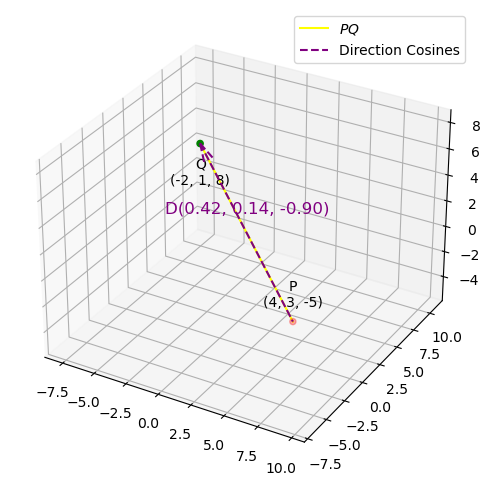
\includegraphics[width=1\textwidth]{plots/plot.png}
    \caption{ Line PQ}
    \label{fig:plot}
\end{figure}   
   }
\end{document}


